\documentclass[border=2pt]{standalone}
\usepackage{pgfplots}
\pgfplotsset{compat=1.18}

\begin{document}

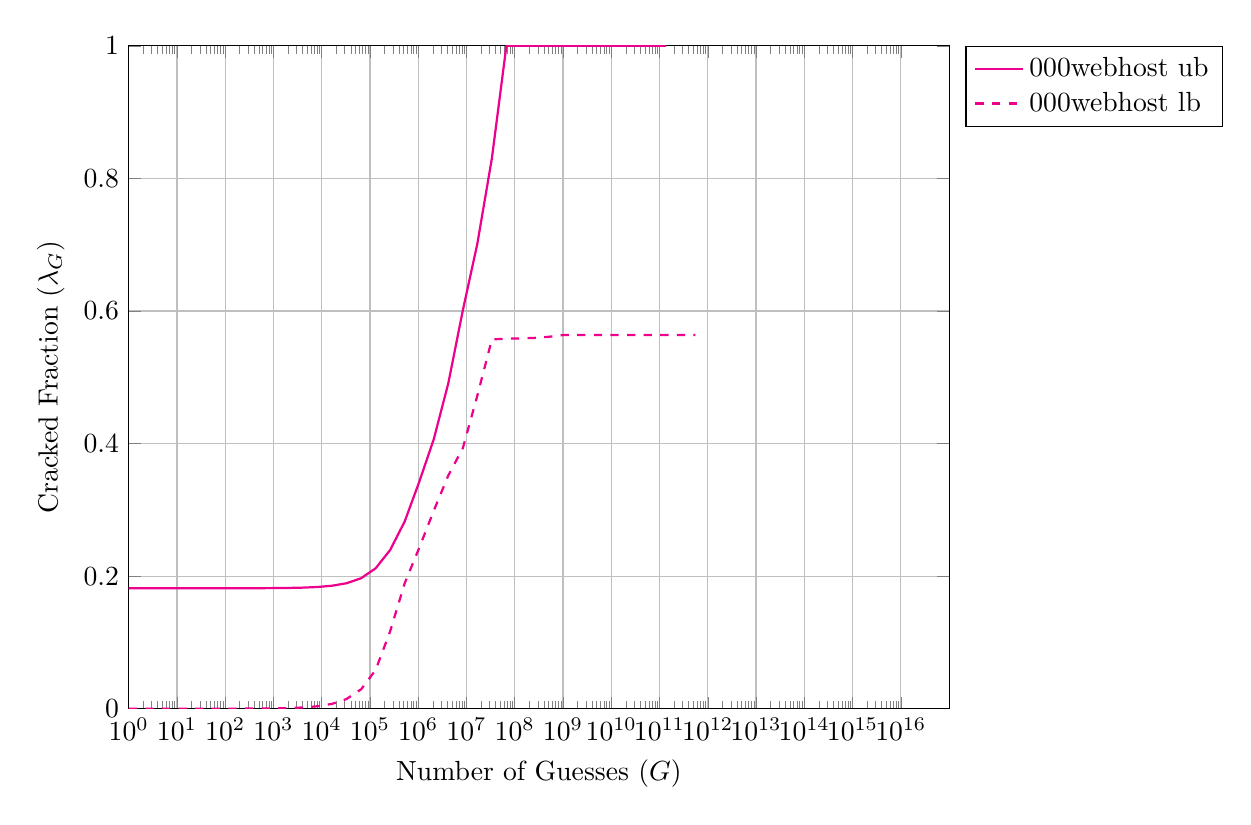
\begin{tikzpicture}
  \begin{axis}[
    width=12cm,
    height=10cm,
    xmode=log,
    xmin=1, xmax=1e17,
    xtick={1,10,100,1000,10000,100000,1000000,10000000,100000000,1000000000,10000000000,100000000000,1000000000000,10000000000000,100000000000000,1000000000000000,10000000000000000},
    xticklabels={$10^{0}$,$10^{1}$,$10^{2}$,$10^{3}$,$10^{4}$,$10^{5}$,$10^{6}$,$10^{7}$,$10^{8}$,$10^{9}$,$10^{10}$,$10^{11}$,$10^{12}$,$10^{13}$,$10^{14}$,$10^{15}$,$10^{16}$},
    ymin=0.0, ymax=1.0,
    xlabel={Number of Guesses ($G$)},
    ylabel={Cracked Fraction ($\lambda_G$)},
    grid=major,
    legend style={at={(1.02,1)}, anchor=north west},
    legend cell align={left},
    legend columns=1,
  ]

% 000webhost UB Data
\addplot[magenta, solid, thick] coordinates {
(1, 0.181676) (2, 0.181676) (4, 0.181676) (8, 0.181677) 
(16, 0.181678) (32, 0.181682) (64, 0.18169) (128, 0.181704) 
(256, 0.181734) (512, 0.181794) (1024, 0.181912) (2048, 0.18215) 
(4096, 0.182625) (8192, 0.183575) (16384, 0.185473) (32768, 0.189264) 
(65536, 0.196821) (131072, 0.211786) (262144, 0.239477) (524288, 0.282503) 
(1.04858e+06, 0.342241) (2.09715e+06, 0.406493) (4.1943e+06, 0.490854) (8.38861e+06, 0.600887) 
(1.67772e+07, 0.701565) (3.35544e+07, 0.83018) (6.71089e+07, 1) (1.34218e+08, 1) 
(2.68435e+08, 1) (5.36871e+08, 1) (1.07374e+09, 1) (2.14748e+09, 1) 
(4.29497e+09, 1) (8.58993e+09, 1) (1.71799e+10, 1) (3.43597e+10, 1) 
(6.87195e+10, 1) (1.37439e+11, 1) 
};
\addlegendentry{000webhost ub}

% 000webhost LB Data
\addplot[magenta, dashed, thick] coordinates {
(1, 4.46059e-07) (2, 8.92117e-07) (4, 1.78423e-06) (8, 3.56847e-06) 
(16, 7.13694e-06) (32, 1.42739e-05) (64, 2.85478e-05) (128, 5.70955e-05) 
(256, 0.000114191) (512, 0.000228382) (1024, 0.000456764) (2048, 0.000913528) 
(4096, 0.00182706) (8192, 0.00365411) (16384, 0.00730823) (32768, 0.0146165) 
(65536, 0.0292329) (131072, 0.0584658) (262144, 0.116932) (524288, 0.189303) 
(1.04858e+06, 0.242746) (2.09715e+06, 0.298702) (4.1943e+06, 0.35177) (8.38861e+06, 0.393001) 
(1.67772e+07, 0.472306) (3.35544e+07, 0.557138) (6.71089e+07, 0.558137) (1.34218e+08, 0.558575) 
(2.68435e+08, 0.559452) (5.36871e+08, 0.561207) (1.07374e+09, 0.563868) (2.14748e+09, 0.563868) 
(4.29497e+09, 0.563868) (8.58993e+09, 0.563868) (1.71799e+10, 0.563868) (3.43597e+10, 0.563868) 
(6.87195e+10, 0.563868) (1.37439e+11, 0.563868) (2.74878e+11, 0.563868) (5.49756e+11, 0.563868) 
};
\addlegendentry{000webhost lb}

  \end{axis}
\end{tikzpicture}

\end{document}